\section{User Interface}

Für das User-Interface wurde das JavaScript-Framework Angular verwendet. 
Diese Entscheidung fiel auf Angular, da es über eine umfassende Dokumentation verfügt und 
sich ideal für die Entwicklung von Webanwendungen eignet. Außerdem waren die 
Teammitglieder mit diesem Framework am vertrautesten, was die Entwicklung und Zusammenarbeit 
erheblich erleichterte. \\

\noindent Im Bereich JavaScript besteht die Möglichkeit, Pakete von anderen Entwicklern zu nutzen. 
Diese Pakete können mithilfe eines Paket-Managers wie \textit{npm} installiert werden. 
In diesem Projekt haben wir das Design-Framework \textit{Project Clarity} und das 
Chart-Framework \textit{chart.js} über \textit{npm} installiert. Eine ausführlichere Betrachtung des 
Designs erfolgt im entsprechenden Abschnitt. \\

\noindent Das User-Interface ist in verschiedene Seiten unterteilt. Eine detaillierte Betrachtung der 
einzelnen Seiten erfolgt im Abschnitt \textit{Seiten}. Die allgemeine Navigationsstruktur wird im 
Abschnitt \textit{Navigation} ausführlich erläutert.

\notebox {
Für die prototypische Entwicklung wurde das User-Interface in englischer Sprache erstellt. 
Für die finale Version des User-Interfaces ist eine Übersetzung in verschiedene Sprachen erforderlich, 
um eine größere Nutzergruppe anzusprechen. Dabei können Pakete wie \textit{ngx-translate} verwendet werden.
}

\subsection{Design}

Für die Entwicklung des User-Interfaces wurde das Design-Framework \textit{Project Clarity} verwendet. 
Dieses Framework bietet eine breite Palette von vorgefertigten Komponenten, die sich leicht in das +
User-Interface integrieren lassen.

\notebox {
Für die prototypische Entwicklung des User-Interfaces verwendeten wir das Design-Framework
\textit{Project Clarity}. Für die endgültige Version des User-Interfaces ist eine Anpassung des 
Designs an das Corporate Design der Hochschule erforderlich, um eine konsistente Benutzererfahrung 
sicherzustellen.
}

\noindent Zur Darstellung von Diagrammen haben wir das Chart-Framework \textit{chart.js} verwendet. 
Dieses Framework bietet eine breite Auswahl an Diagrammtypen, die sich einfach in das 
User-Interface integrieren lassen. Diese Diagramme sind auf dem User-Dashboard und dem 
Team-Dashboard eingebunden.

\subsection{Navigation}

Die Navigation des User-Interfaces ist in zwei Bereiche unterteilt. 
Der erste Bereich ist die Navigationsleiste, die sich am oberen Rand des User-Interfaces befindet. 
In dieser Navigationsleiste finden sich Links zu den verschiedenen Seiten des User-Interfaces, 
darunter das User-Dashboard, die Team- und Quiz-Übersicht. Außerdem gibt es in der 
Navigationsleiste einen Link zum User-Profil und einen Link zum Logout.

\begin{figure}[H]
  
\includegraphics[width=\linewidth]{img/navbar.png}
  \caption{Navigationsbar}
  \label{fig:navbar}
\end{figure}

\noindent Der zweite Abschnitt der Navigation ist die Suchleiste in der oberen Navigationsleiste. 
Hier kann mittels einer Volltextsuche nach Teams und Quizzen gesucht werden, und die Ergebnisse 
können direkt aufgerufen werden.

\begin{figure}[H]
  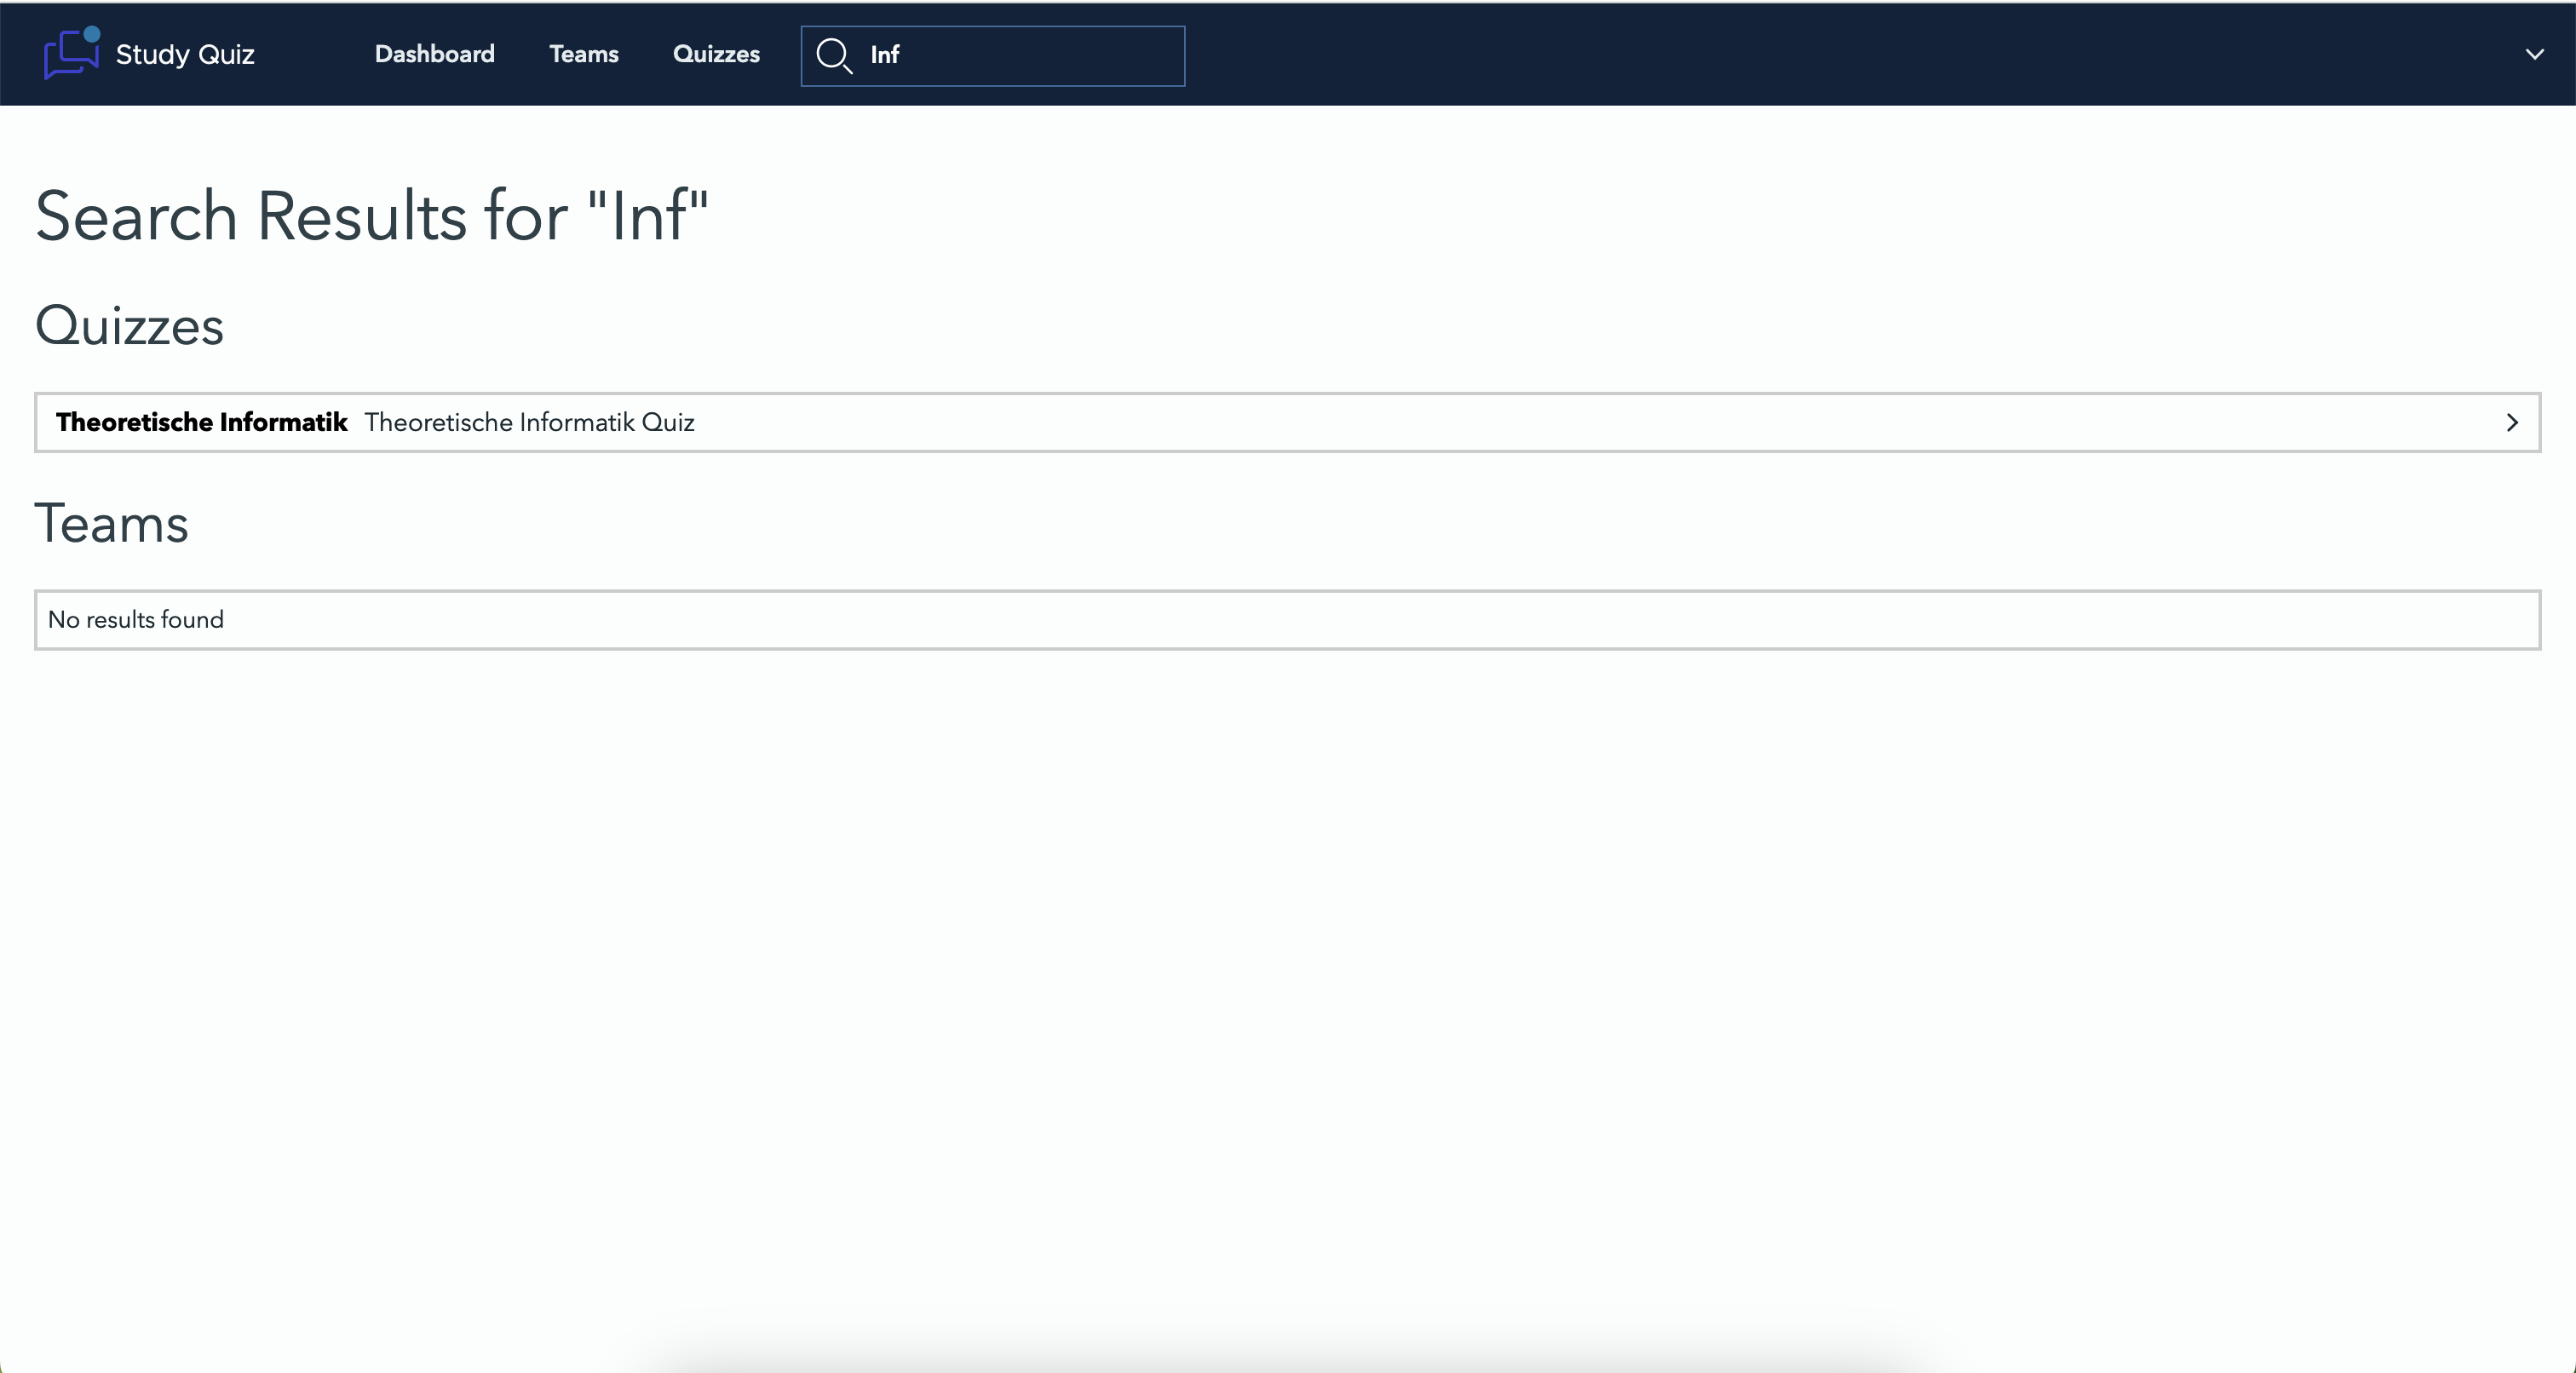
\includegraphics[width=\linewidth]{img/suche.png}
  \caption{Search-Page}
  \label{fig:searchbar}
\end{figure}
\subsection{Seiten}

\subsection*{Login \& Registrierung}

\noindent Die Login-Seite bietet dem Benutzer die Möglichkeit, sich am System anzumelden. 
Auf der linken Seite der Login-Seite kann der Benutzer seinen Benutzernamen und sein Passwort 
eingeben. Wenn diese korrekt sind, wird eine Bestätigung angezeigt, und der Benutzer wird nach 
zwei Sekunden zum Nutzer-Dashboard weitergeleitet. \\

\noindent Wenn ein Benutzer versucht, auf eine Seite der Webanwendung zuzugreifen, 
ohne angemeldet zu sein, wird er automatisch zur Anmeldeseite weitergeleitet.

\begin{figure}[H]
  
\includegraphics[width=\linewidth]{img/login.png}
  \caption{Login Seite}
  \label{fig:login}
\end{figure}

\noindent Über den unteren Link auf der Login-Seite kann ein Nutzer ohne Benutzerkonto zur 
Anmeldeseite gelangen. Dort muss er im Formular seinen gewünschten Benutzernamen, 
seine E-Mail-Adresse und ein Passwort eingeben. Sobald das Formular validiert ist, 
kann der 'Registrieren'-Button gedrückt werden. Bei erfolgreicher Registrierung wird 
dem Nutzer eine Bestätigung angezeigt, und er wird nach zwei Sekunden zur Anmeldeseite 
weitergeleitet, wo er sich mit seinem neu erstellten Nutzerkonto anmelden kann.

\begin{figure}[H]
  
\includegraphics[width=\linewidth]{img/register.png}
  \caption{Registrierungs Seite}
  \label{fig:register}
\end{figure}

\subsection*{Dashboard}

Das Nutzer-Dashboard ist die personalisierte Seite für den Nutzer und wird ihm unmittelbar nach 
der Anmeldung angezeigt. \\

\noindent Im oberen Bereich des Dashboards wird dem Nutzer auf der linken Seite sein aktueller Punktestand für 
den aktuellen Monat angezeigt. Dieser Punktestand repräsentiert die in diesem Monat erzielten Quiz-Punkte. 
Auf der rechten Seite kann der Nutzer mithilfe eines Graphen seine monatlichen Punktzahlen der 
vergangenen Monate analysieren. \\

\noindent Im mittleren Bereich des Dashboards hat der Nutzer Zugriff auf seine zehn zuletzt durchgeführten Quizze. 
Wenn ein Quiz nicht abgeschlossen wurde, kann der Nutzer es durch einen Klick auf das Quiz fortsetzen. \\

\noindent Im unteren Bereich des Dashboards befindet sich der Leaderboard-Bereich. Hier werden auf der linken Seite 
die zehn Nutzer mit den meisten Punkten in diesem Monat und auf der rechten Seite die zehn Teams mit 
den meisten Punkten in diesem Monat angezeigt. \\

\noindent Das Nutzer-Dashboard kann über den Navigationspunkt "Dashboard" von jeder Seite der Webanwendung 
aus erreicht werden. \\


\begin{figure}[H]
  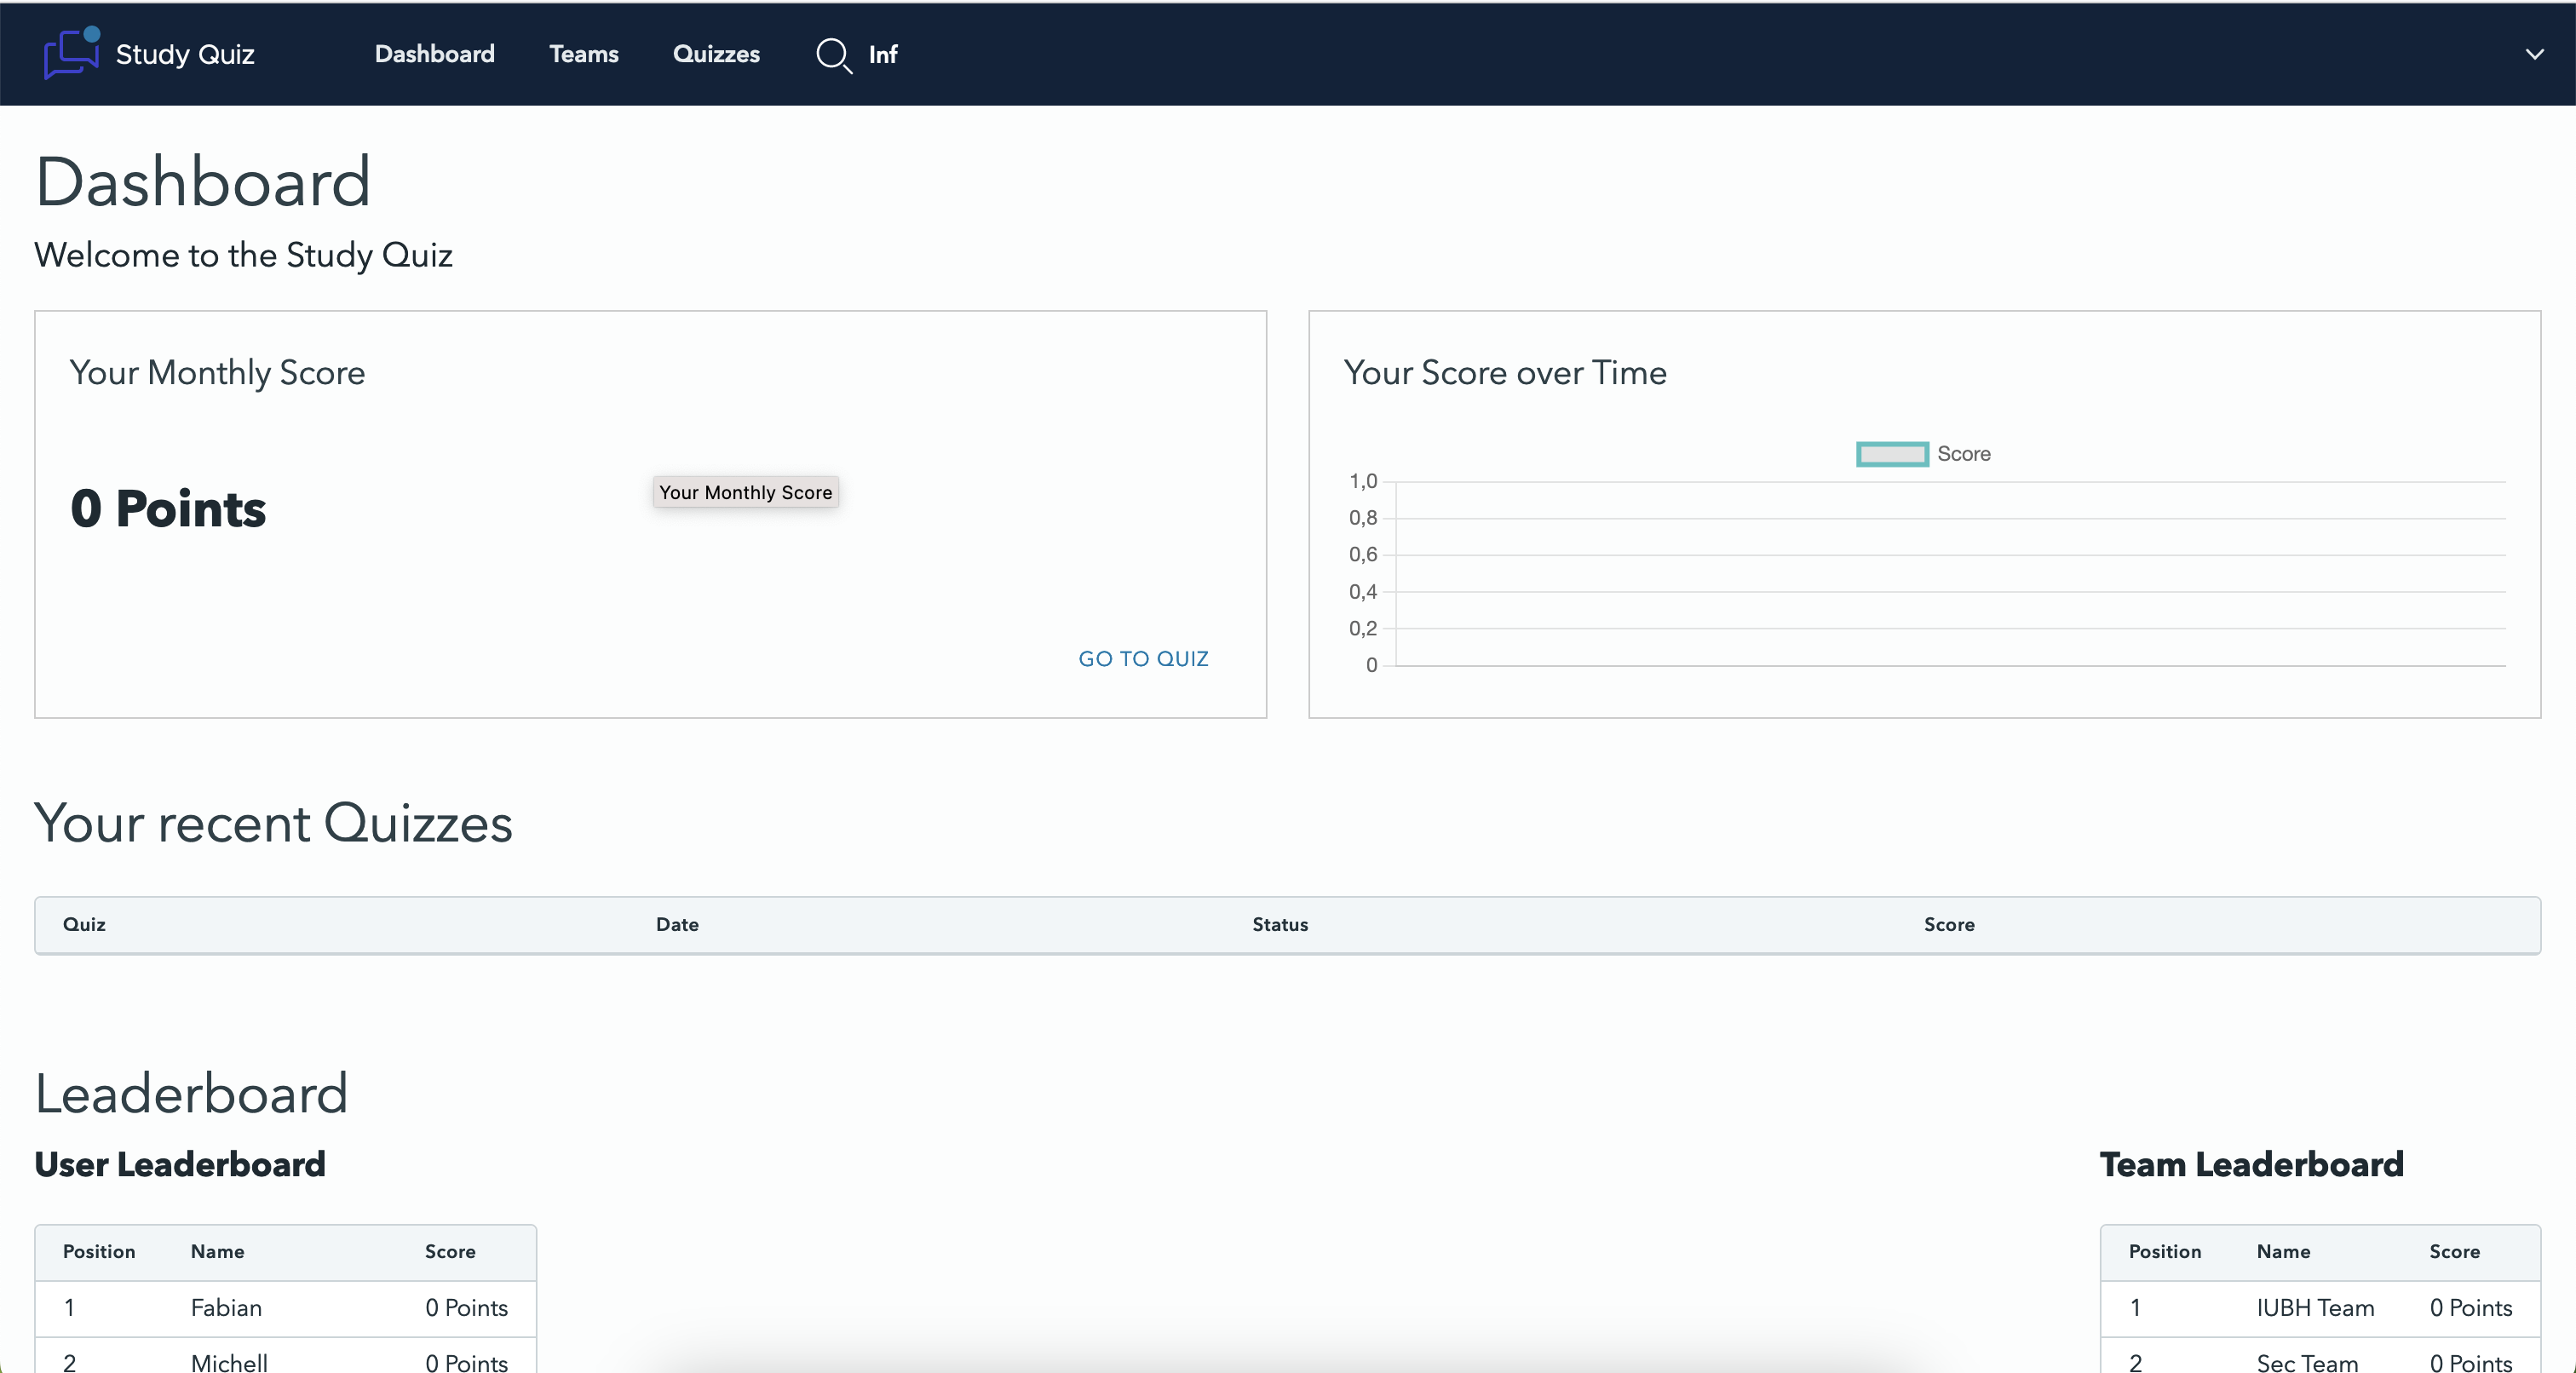
\includegraphics[width=\linewidth]{img/dashboard.png}
  \caption{Dashboard Seite}
  \label{fig:dashboard}
\end{figure}

\subsection*{Quiz Seiten}

Die Quiz-Übersicht kann über die Navigationsleiste unter dem Punkt \textit{Quizzes} 
von jeder Seite der Webanwendung aus erreicht werden. Sie enthält eine Liste aller verfügbaren 
Quizze in der Anwendung.

\begin{figure}[H]
  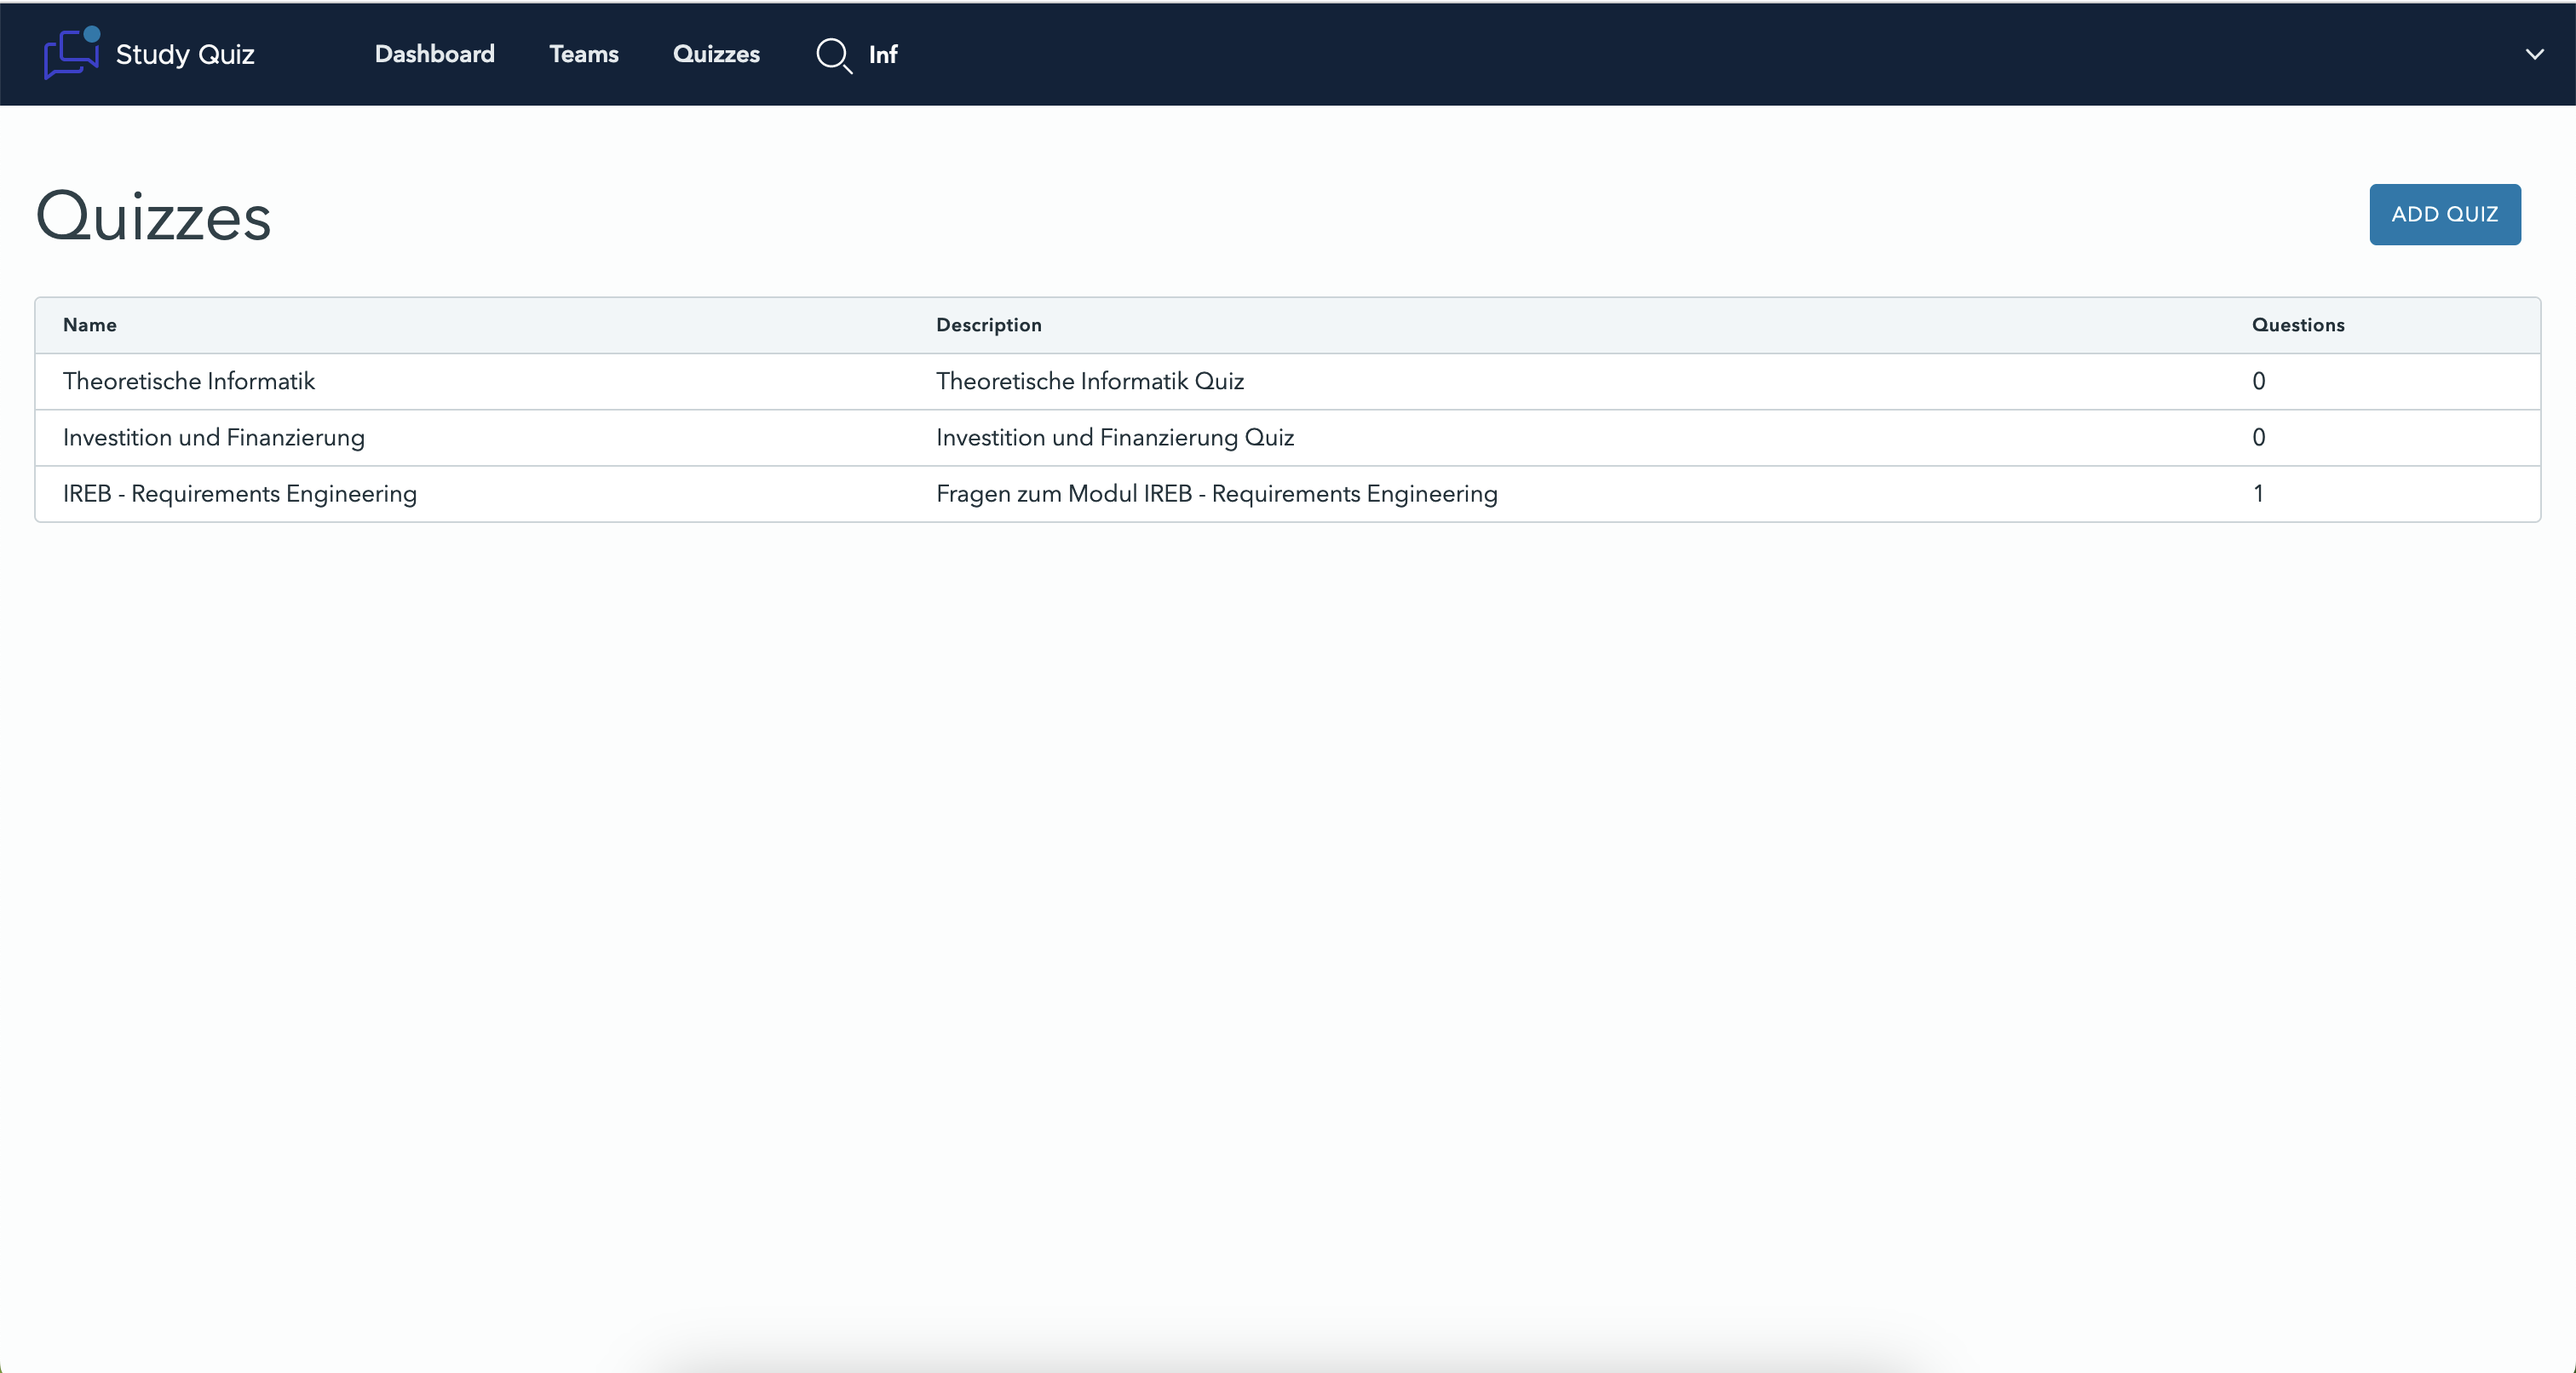
\includegraphics[width=\linewidth]{img/quiz-list.png}
  \caption{Quiz-Übersichtsseite}
  \label{fig:quiz}
\end{figure}

\noindent Um zum Quiz-Dashboard zu gelangen, wählen Sie in der Quiz-Übersichtsseite eines der Quizze aus. \\

\noindent Im oberen Bereich des Quiz-Dashboards finden Sie auf der linken Seite allgemeine Informationen 
zum Quiz, wie den Quiznamen, die Beschreibung sowie den Ersteller und das Erstellungsdatum. 
Auf der rechten Seite befindet sich der Button "Quiz durchführen", über den Sie eine Quiz-Sitzung 
starten können. Dieser Button ist jedoch erst aktiv, wenn mindestens zehn Fragen in dem Quiz erstellt 
wurden. Außerdem stehen Edit- und Delete-Buttons zur Verfügung, die nur dem Quiz-Ersteller angezeigt 
werden, da nur dieser das Quiz umbenennen oder löschen kann. \\

\noindent Unterhalb des Header-Bereichs des Quiz-Dashboards wird eine Liste von Fragen angezeigt. 
Hier werden die Quiz-Fragen des Quizzes angezeigt und können von jedem Benutzer bearbeitet
und gelöscht werden. Über den "Add Question"-Button kann ein Benutzer dem Quiz eine neue Frage hinzufügen. \\

\noindent Im unteren Bereich der Seite werden die letzten Versuche angezeigt, jeweils mit ihrem Status und Score.


\begin{figure}[H]
  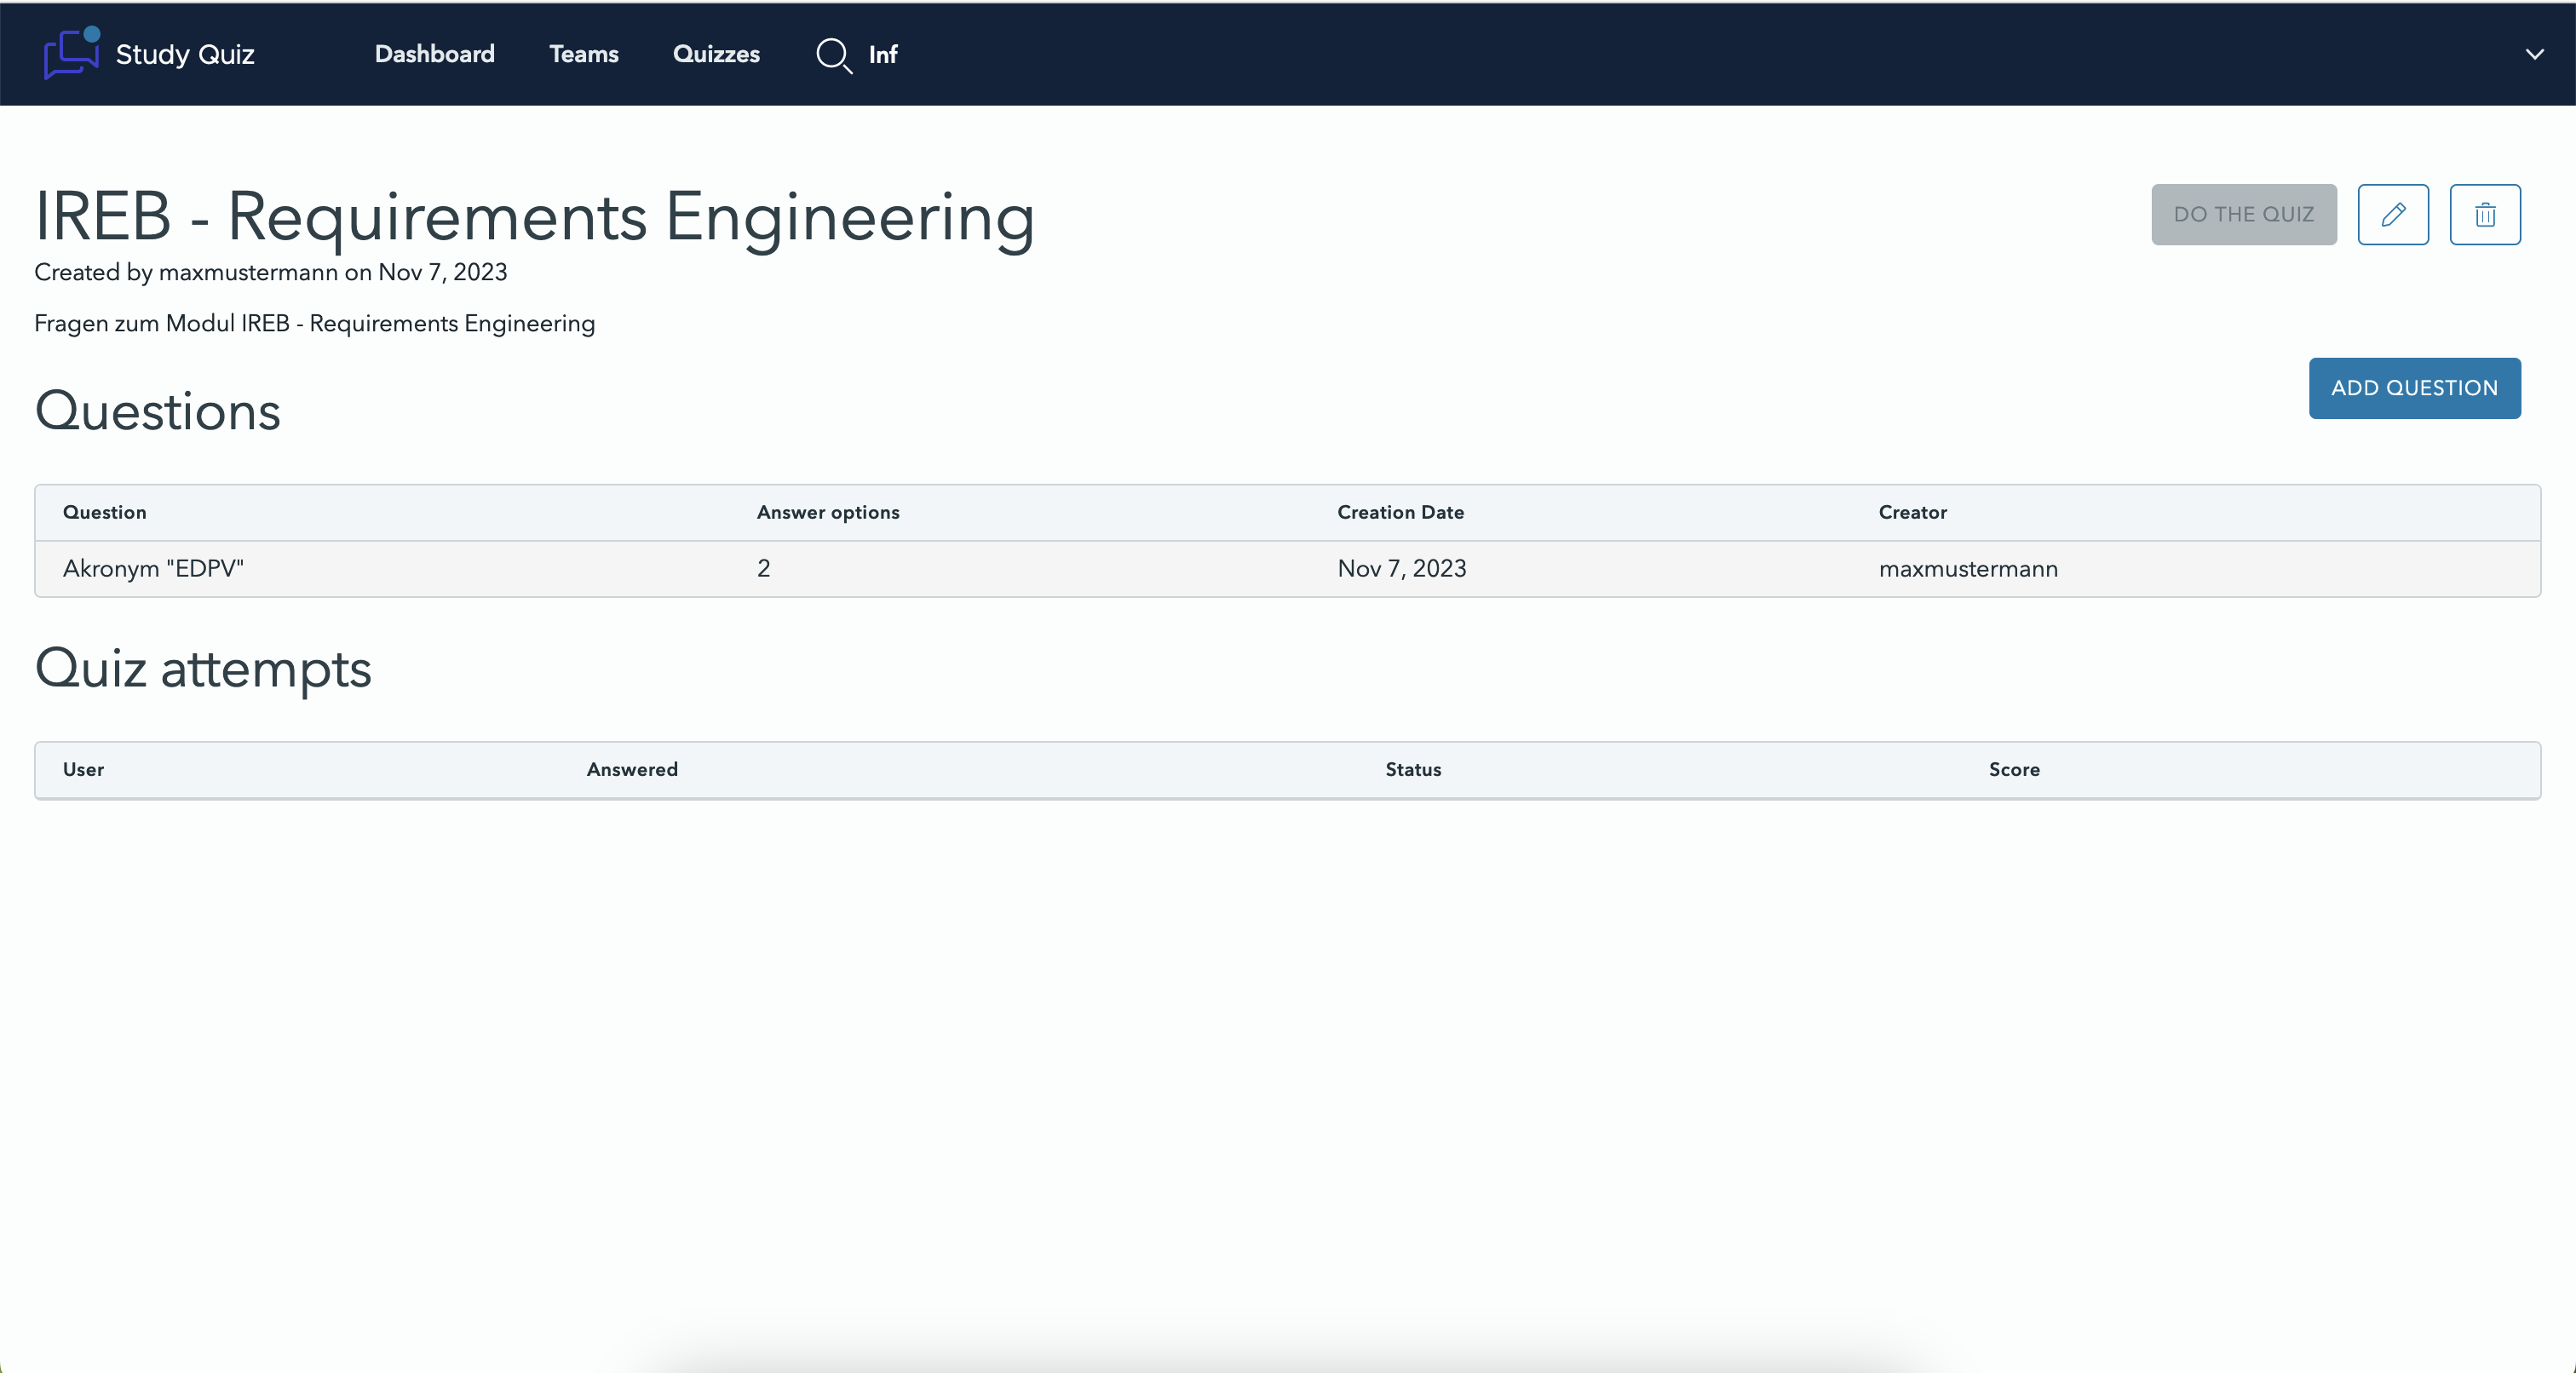
\includegraphics[width=\linewidth]{img/quiz-detail.png}
  \caption{Quiz-Dashboard}
  \label{fig:quiz}
\end{figure}

% TODO: Add Do-Quit Page

\subsection*{Team Seiten}

Die Teams-Übersichtsseite kann direkt über den Navigationspunkt \textit{Teams} in der 
Navigationsleiste aufgerufen werden. Auf dieser Seite werden alle Teams des Systems aufgelistet.
Durch einen Klick auf ein Team gelangt man zum Team-Dashboard.

\begin{figure}[H]
  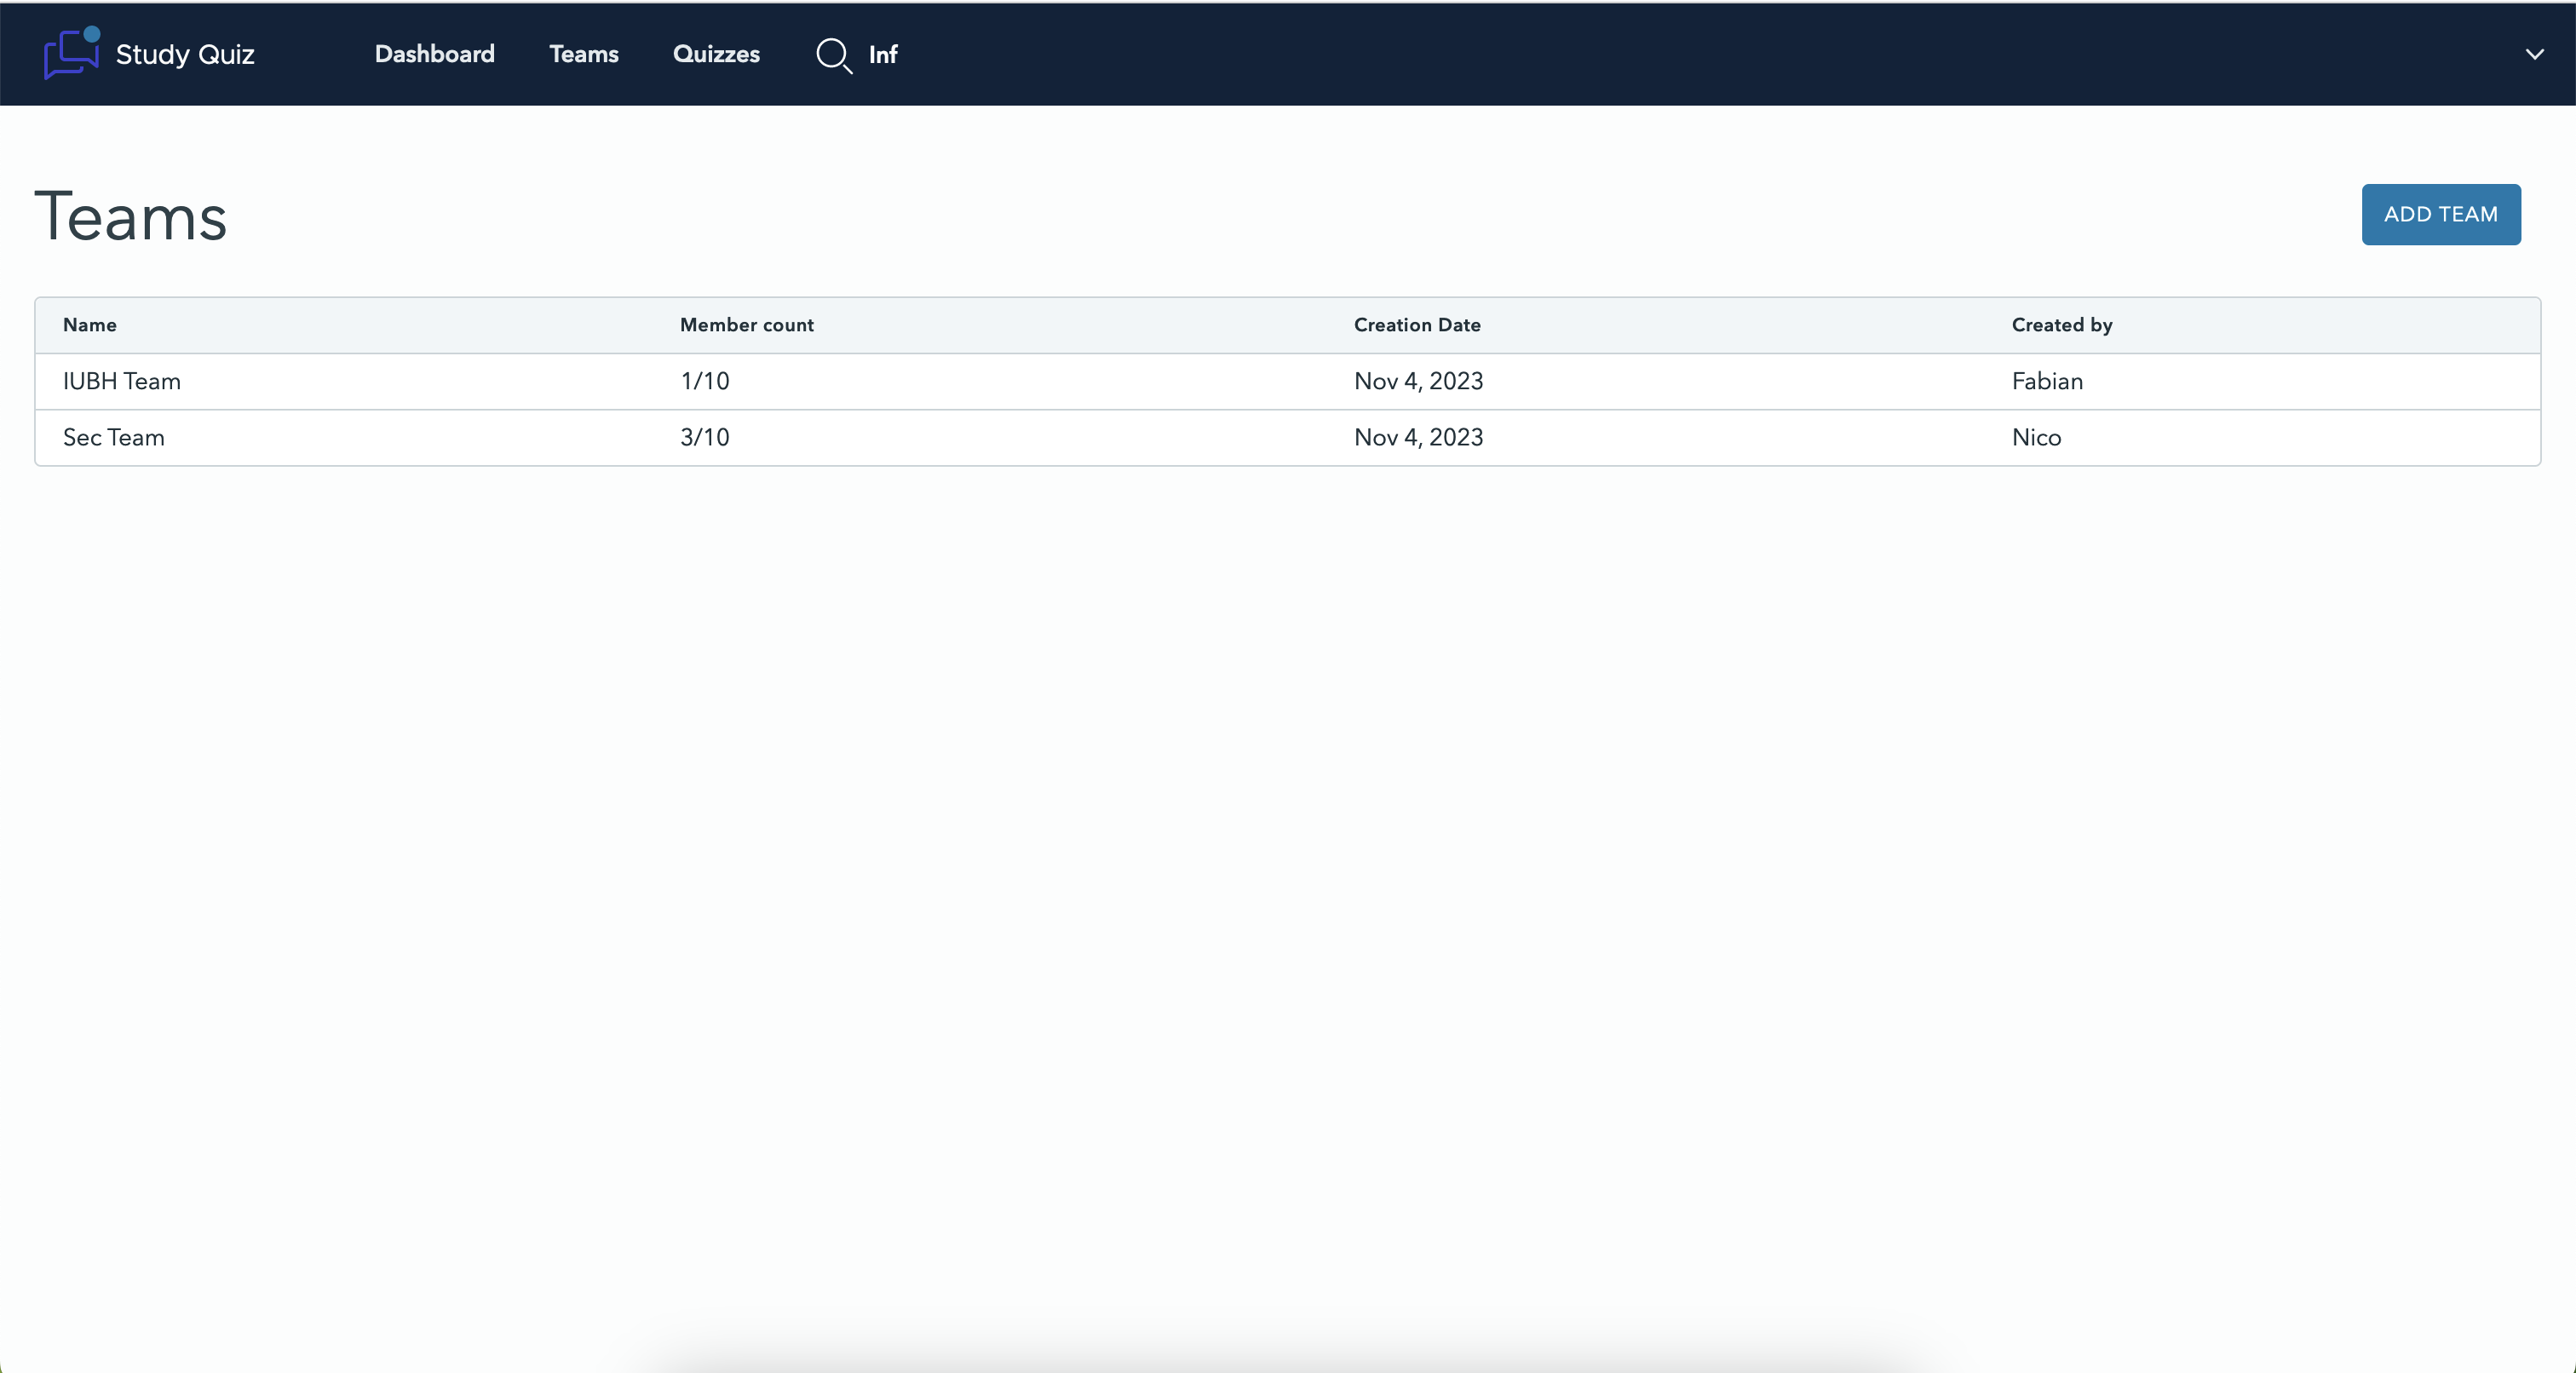
\includegraphics[width=\linewidth]{img/team-list.png}
  \caption{Teams Übersichtsseite}
  \label{fig:team}
\end{figure}

\noindent Auf der Team-Dashboard-Seite befinden sich im oberen linken Bereich die Grundinformationen zu dem 
ausgewählten Team, wie Name, Mitgliederanzahl, Ersteller und Erstellungsdatum. Im rechten Bereich befindet 
sich ein Button mit der Bezeichnung \textit{Join}, über den Nutzer dem Team beitreten können. 
Dieser Button ist nur solange aktiv, wie das Team noch freie Plätze hat.

\notebox {
  Eine sinnvolle Erweiterung für eine potenzielle Produktivumsetzung wäre die Möglichkeit, ein Team mit einem Passwort zu schützen, so dass nur eingeladene Nutzer, die das Passwort haben, dem Team beitreten können.
}

\noindent Unterhalb des Header-Bereichs des Team-Dashboards sind die aktuellen Statistiken des Teams sichtbar. 
Auf der linken Seite wird der aktuelle Teamscore angezeigt, der die Summe der User-Scores aller 
Mitglieder darstellt. Auf der rechten Seite befindet sich ein Graph, der den Teamscore über die Zeit 
darstellt. \\

\noindent Darunter befindet sich ein Abschnitt, in dem die zuletzt erzielten Scores der Mitglieder aufgelistet sind. \\

\noindent Darunter befindet sich eine Tabelle mit allen Mitgliedern in diesem Team. \\

\noindent Im Allgemeinen besteht ein Team aus maximal 10 Mitgliedern. Nur der Ersteller des Teams hat die 
Berechtigung, das Team zu bearbeiten oder zu löschen. Der Ersteller des Teams kann auch Teilnehmer 
aus dem Team entfernen.

\begin{figure}[H]
  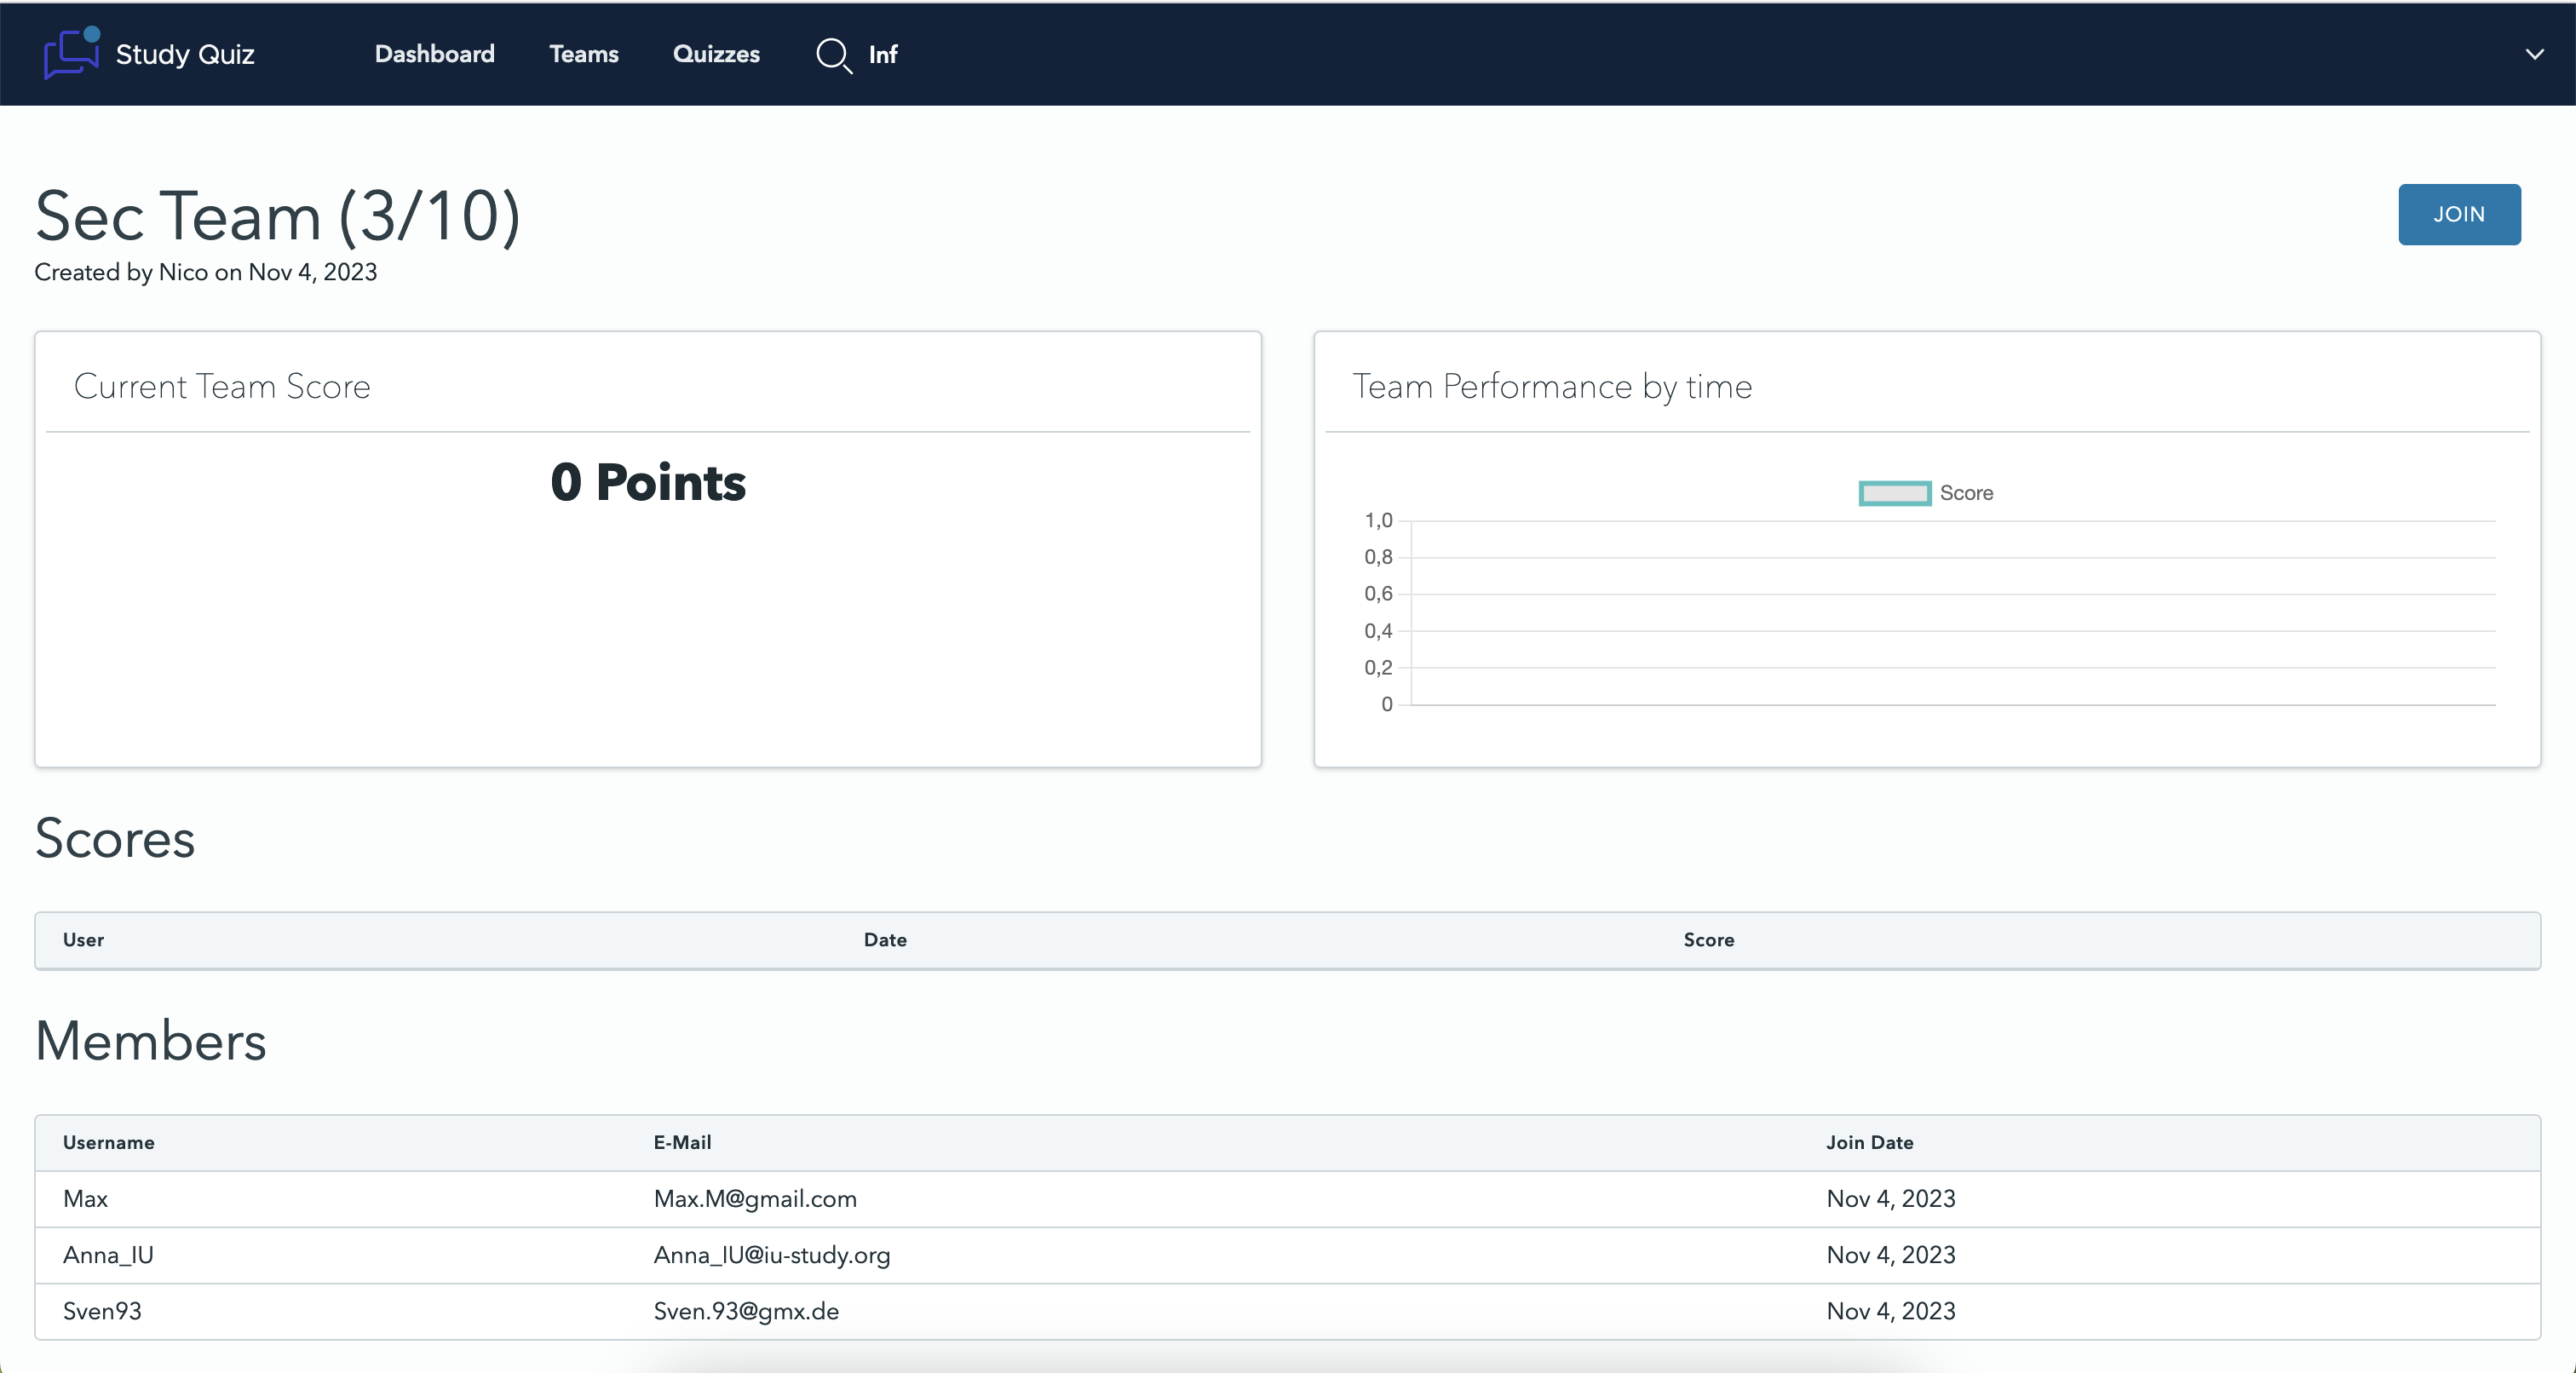
\includegraphics[width=\linewidth]{img/team-detail.png}
  \caption{Team-Dashboard}
  \label{fig:team}
\end{figure}
